\section{Compiler Overview (Ready)}

\begin{figure*}
\centering
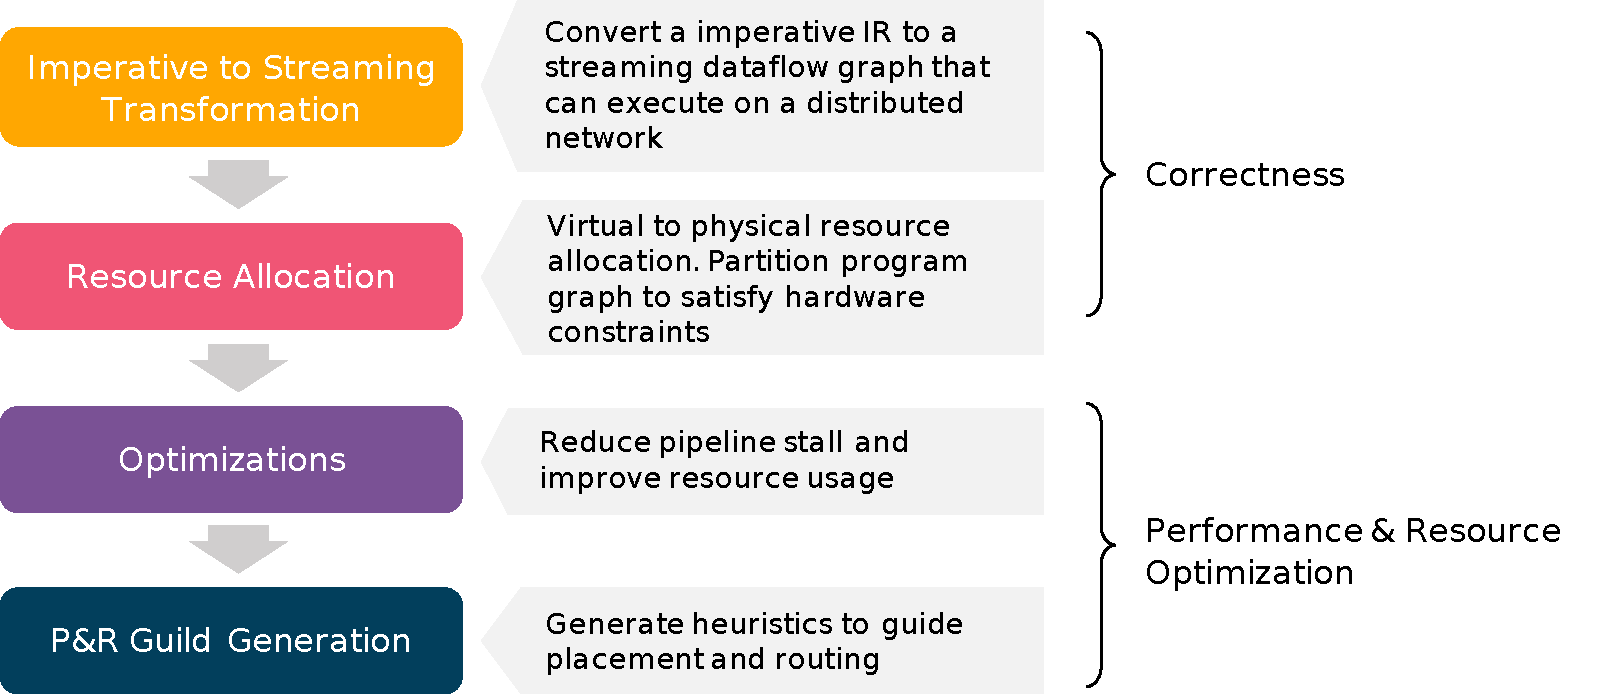
\includegraphics[width=1\textwidth]{figs/sarastack.pdf}
\caption[\name Compiler Flow]{\name Compiler Flow}
\label{fig:flow}
\end{figure*}
 
In this section, we describe a systematic approach to compile applications described in an
imperative front-end language with a purely declarative and distributed dataflow graph that can
run on Plasticine.
\Cref{fig:flow} shows the compilation flow to perform this translation between the two paradigms.
At high-level, \name allocates distributed on-chip resources to execute the program in spatially parallelized and
pipelined fashion.
\name automatically generates synchronization across distributed units to provide strong memory consistency for an imperative program, on an architecture that does not guarantee memory
ordering across multiple access streams.
This synchronization is purely point-to-point, introducing minimum performance overhead, which
maximizes the scalability of the architecture.
\name further virtualizes resource allocation and hides the underlying resource constrains on
this hierarchical architecture from the programmers.

First, \name takes the input Spatial IR and performs the \term{imperative to streaming
transformation}.
A virtual unit (VU) is our intermediate representation that captures computations 
%that will be
%mapped onto 
within the boundary of
a physical unit (PU), such as a PCU and PMU.
Each VU can contain multiple contexts, if their aggregated resources usage can fit in a PU.
The hardware can limit the maximum number of contexts a PU can support and has resources that cannot be split across contexts.
Additionally, messages across VUs are mapped across the global network, which must tolerate an arbitrary amount of network latencies; messages within a single VU across contexts takes only a single cycle.
The transformation phase generates a virtual unit dataflow graph (VUDFG) with appropriate
synchronizations, such that a streaming pipelined execution over distributed on-chip resources produces the same result as a
parallelized program executed in time.

At the end of the allocation phase, a virtual unit can consume as much resources as the program
requires. The second phase is \term{resource allocation}, where \name assign each VU to a
PU that processes the required resources. If no PU can execute a VU, \name partitions the
VU into multiple VUs to eliminate constraint violations. If there is insufficient PU or the VU cannot be partitioned, the mapping process fails with appropriate hints to the programmer for the
limiting resources.

Throughout the first two phases, \name introduces various \term{optimizations} that either reduce the
resource cost of the VUDFG, or alleviates potential performance bottleneck in the streaming
pipeline.
After all VU fits in at least one type of PU, \name performs a global optimization that merges small VUs into a larger VU to reduce resource fragmentations.

The output of the resource allocation phase is a VUDFG with a tagged PU type for each VU.
It is up to the
\term{placement and routing (PaR)} phase to determine where the VU will be finally placed.
Right before PaR, \name performs static analysis on the traffic pattern and generate heuristic guild
for the placer to reduce routing congestion.

